\section{Resultats}

\subsection{Determinació del transitori}

El procés de càlcul del transitori és un poc bast però efectiu: calculàrem
distintes traces per un nombre de clients suficientment gran (100, 200, 250 i
300) i estudiàrem a partir de quin punt el sistema es comportava de manera
estable o cíclica. Com a regla general vàrem poder apreciar que obtenint uns
vint esdeveniments per client i quedant-nos sols amb la segona meitat de tota
la simulació els resultats eren estables.

A les gràfiques es mostra la tendència dels temps de resposta al llarg d'una
simulació.

\newcommand{\grafictransitori}[2]{
\begin{figure}[t]
  \centering
  \includegraphics[width=\textwidth]{img/evo-#1.png}
  \caption{Execució amb #1 clients per estudiar el transitori}
  \includegraphics[width=\textwidth]{img/evo-#2.png}
  \caption{Execució amb #2 clients per estudiar el transitori}
\end{figure}
}

\grafictransitori{100}{200}
\grafictransitori{250}{300}

\subsection{Càlcul de temps de resposta}

Per determinar el punt d'inflexió del nostre sistema calcularem els distints
temps de resposta a mida que anam aumentant els clients. Els temps de resposta
de les simulació es poden llegir a la figura ~\ref{resultats:temps:taula} i es
poden veure representats en la gràfica ~\ref{resultats:temps:grafica}.


\begin{figure}
\centering
\begin{tabular}{lrlr}
N usuaris & TR (ms) &
N usuaris & TR (ms) \\

\toprule

10    & 42.08    &  
260   & 1573.98  \\ 
20    & 42.26    &  
270   & 1961.58  \\
30    & 44.75    &  
280   & 2334.91  \\ 
40    & 49.49    &  
290   & 2688.70  \\
50    & 56.00    &  
300   & 3060.17  \\ \midrule
60    & 56.66    &  
310   & 3421.07  \\
70    & 63.94    &  
320   & 3809.61  \\  
80    & 63.48    &  
330   & 4203.65  \\ 
90    & 66.70    &  
340   & 4591.56  \\ 
100   & 75.61    &  
350   & 4983.98  \\ \midrule
110   & 73.92    &  
360   & 5382.18  \\ 
120   & 87.58    &  
370   & 5762.88  \\
130   & 84.71    &  
380   & 6181.55  \\ 
140   & 91.32    &  
390   & 6584.32  \\
150   & 110.19    &  
400   & 6949.67  \\ \midrule
160   & 110.71    &  
410   & 7346.90  \\
170   & 120.57    &  
420   & 7755.98  \\ 
180   & 137.82    &  
430   & 8086.00  \\
190   & 190.46    &  
440   & 8511.05  \\ 
200   & 254.08    &  
450   & 8891.28  \\ \midrule
210   & 356.87    &  
460   & 9328.79  \\ 
220   & 484.69    &  
470   & 9732.96  \\
230   & 624.87    &  
480   & 10146.00  \\ 
240   & 748.87    &  & \\
250   & 1198.98  &  & \\ 

\bottomrule

\end{tabular}
  \caption{Evolució dels temps de resposta segons es van afegint
    usuaris. Aquestes simulacions són de rèpliques.}

  \label{resultats:temps:taula}

\end{figure}


\begin{figure}
  \centering
  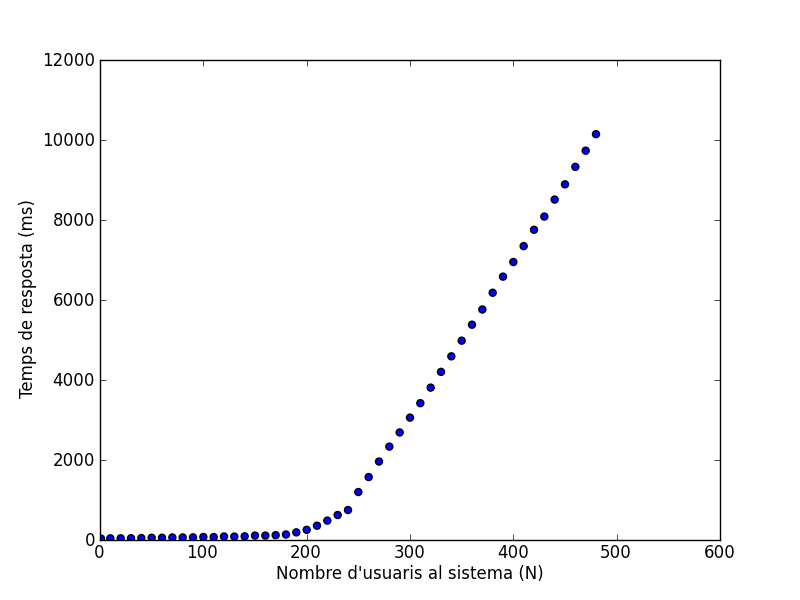
\includegraphics[width=\textwidth]{img/sim.png}

  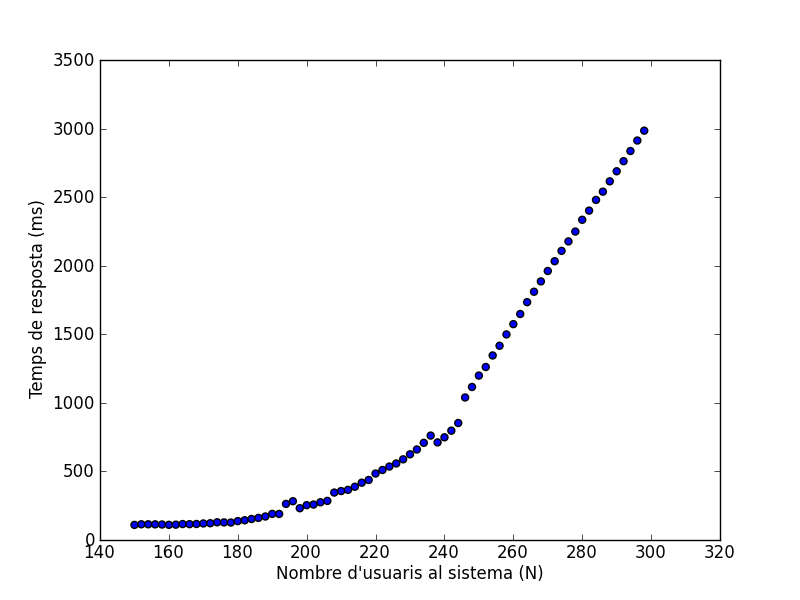
\includegraphics[width=\textwidth]{img/sim-retall-150-300.png}

  \caption{Evolució dels temps de resposta segons es van afegint usuaris en
    simulacions mitjançant rèpliques.}
  \label{resultats:temps:grafica}

\end{figure}

Després de les simulacions podem observar i concloure que:

\begin{enumerate}

  \item Sols hem utilitzat un processador pel nostre servidor, de temps de
    servei $0.4ms$.

  \item El disc té un temps de servei de casi $8ms$.

  \item Una operació demana una mitja de cinc transaccions de disc.

  \item Fins als 200 usuaris el sistema manté un temps de resposta d'un quart
    de segon ($250ms$), rendiment acceptable per una aplicació interactiva.

  \item A partir dels 250 usuaris l'aplicació passa a tenir un temps de
    resposta d'un segon, fent-la adient sols per aplicacions no purament
    interactives.

  \item Des dels 200 usuaris, afegint un 0.25 de càrrega hem quadruplicat el
    temps de resposta. Podem afirmar que entre el rang de 200 i 250 usuaris
    tenim el punt d'inflexió del sistema.

  \item Malgrat no tinguem els càlculs de l'utilització de la CPU, la
    diferència de magnitud de temps de resposta amb el disc (vint vegades) ens
    indica que probablement el coll de botealla és el disc.

\end{enumerate}

\paragraph{Conclusions}

Recordant que hem modelat un sistema amb un processador i un disc modern i
potent podem veure el gran nombre d'usuaris que s'han de menester per saturar
el sistema. El coll de botella és el disc dur doncs és casi vint vegades més
lent que el processador. De tota manera cal recordar que si consideràssim un
temps de resposta inacceptable a partir del segon ja estam parlant de casi 250
usuaris concurrents per un conjunt \emph{hardware} que no arriba ni als 1000€.

D'aquesta manera i malgrat hem fet grans simplifiacions, com obviar que els
computadors actuals estan provistos d'un important conjunt de memòries cau, hem
pogut valorar quantitativament el rendiment del sistema i jugar amb el que
podria ser la implementació d'un sistema de simulació.
